\documentclass{csfourzero}

\title{Latency Performance Comparison of Open Source Real-Time Publish-Subscribe Data Distribution Service Implementations}
\author{Marcel Zak}
\date{\today}
% A useful package to support on-line references
\usepackage{url}
\usepackage{natbib}
\usepackage{graphicx}

\bibliographystyle{plain}
\abstract{Will be}


\begin{document}
\maketitle

%\tableofcontents
%\newpage 

\section{Introduction}
\label{sec:intro}

\quad In this research paper I decided to investigate a difference in latency performance in two popular open source implementations of Data Distribution Service (DDS) protocol. DDS is middleware developed by Object Management Group (OMG) \cite{what-is-dds}. It is specifically design as machine to machine, data centric, high performance and reliable protocol. The aim was to create a protocol that does not have a problem with scalability and it fulfils requirements for modern Internet of Things (IoT) applications \cite{DDS-spec}. Later a Real-Time Publish Subscribe (RTPS) DDS was specified as the interoperability protocol. RTPS DDS was designed as real time, low latency protocol for best effort and reliable communication over unreliable transports such as UDP/IP and it is standardized that different RTPS implementations can communicate each other \cite{RTPS-spec}. For its quality and robustness, it is often used in aerospace and defence sectors for real-time applications \cite{eprosima-rtps-intro}. 

For real time applications it is critical to deliver the right message in the right time at the right place. Such systems are widely used in automation, robotics, space industry, medicine and many other places. Time and reliability are one of the most important factors in these systems. Therefore, the right choice of a library is also crucial to the application. 

These two open source libraries implement the same RTPS protocol specification. They are implemented in same programming language C++. The first implementation is OpenDDS \cite{git-openDDS} created by OCI that is a full implementation of DDS. The second library was developed by eProsima and it is standalone RTPS implementation called Fast RTPS \cite{git-eProsima}. It claims to be the fastest one because it is lightweight \cite{eprosima-rtps-intro}. In this paper I will be investigating latency performance of both open source RTPS implementations.

\section{Background and related work}
\label{sec:lit}

\quad As a first thing I describe the underlying design principle behind DDS protocol. Participants (applications) using DDS can publish or subscribe to a specific "topic" of information. A single participant can publish and subscribe to multiple "topics" at the same time. The advantage of DDS against other similar protocols is that it implements rich set of Quality of Service parameters \cite{what-is-dds}. It is possible to set up different aspects of the communication. Be it persistence, reliability, redundancy, transport settings, lifespan and many others. The communication model is not difficult to understand. A topic is a name that refers to a specific piece of information we want to share. It also contains the definition of Data we want to share \cite{eprosima-dds}. See Figure \ref{fig:GlobalDataSpace}.

\begin{figure}[h]
	\centering
	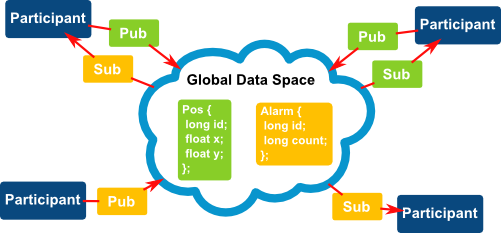
\includegraphics[width=0.6\textwidth]{GlobalDataSpace}
	\caption{\label{fig:GlobalDataSpace}DDS Model: The Global Data Space \cite{eprosima-dds}}
\end{figure}

DDS provide a simple modular design that is shown in Figure \ref{fig:DDSArch}. In these two open source implementation is DDS only a library that is linked to an application. There is no need to install any service or daemon. It is important to note that RTPS is on top of transport layer in the OSI model. Therefore, DDS can be implemented over any kind of underlying transport \cite{eprosima-dds}. DDS specification does not outline how the message should be delivered. Therefore, multiple implementation exist.

\begin{figure}[h]
	\centering
	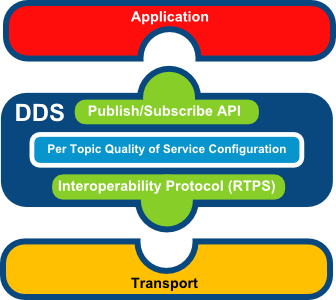
\includegraphics[width=0.5\textwidth]{DDSArch}
	\caption{\label{fig:DDSArch}DDS Architecture \cite{eprosima-dds}}
\end{figure}

I have to say that the scientific community lacks papers about DDS benchmarking. However, there are two papers worth mentioning. The first one is \textit{Performance assessment of OMG compliant data distribution middleware} \cite{omg-perf}. In this paper it is thoroughly discussed the problematic and complexity of benchmarking different DDS implementations. In the second paper \textit{Data Distribution Service (DDS): A performance comparison of OpenSplice and RTI implementations} \cite{splice-vs-rti} is described the process of throughput, latency and CPU load comparison of OpenSplice and RTI DDS implementations.

Authors of the first paper decided to develope a tool called DDSBench that should provide framework for objective performance comparison of different DDS implementations. DDSBench offers variety of possible set-ups such as message type, size, publication period, message iteration, QoS and many others. The idea is that a developer model the test environment based on requirements of the specific application and run the test. Results of the test show which DDS implementation is suitable for the application. It is also discussed different methods for latency measurement. Standard method is \textit{Round-Trip time}. It is the time elapsed between sending a message and receiving it back. However they decided to use \textit{One-way Transit Time} that represent time elapsed between sending the message from publisher to subscriber. The advantage is that it represents more accurately the elapsed time from subscriber's point of view. On the other hand, there is disadvantage and difficulty involved with precise clock synchronisation on both machines  \cite{omg-perf}. I don't agree that for the purpose of benchmarking two implementations is necessary to use \textit{One-way Transit Time}. Based on the related literature \textit{Round-Trip time} reveals the difference in implementations \cite{perf-embedded}. At the end DDSBench is used to evalueate two implementations. The first one is RTI DDS and OpenDDS \cite{omg-perf}. The results clearly showed that the RTI implementation has better performance in all dimensions. I tried to use DDSBench with the newer versions of OpenDDS. Unfortunately, I did not manage to run it probably because the last update of DDSBench was in 2007.

At the beginning of the second paper the DDS standard is well described. The next part focuses on metrics and measurement techniques. Authors decided to measure five different parameters to completely evaluate the performance differences of OpenSplice and RTI implementations. The measured parameters are \textit{Samples per sencon, Throughput, Round-Trip time, CPU and Memory usage}. For latency measurements is used standard \textit{Round-Trip time}. Authors also mentioned that this measurement of latency is widely accepted \cite{perf-embedded}. At the end they performed benchmarking and the results revealed that OpenSplice performs significantly better than RTI in throughput tests and samples per second, but only with messages of smaler size(up to 2048 bytes). If the size of the messages is higher then RTI performs much better. OpenSplice utilizes federated architecture \cite{federated-arch} and by default uses batching optimization this enables better performance for small size data exchange. On the other hand decentralized models (no need for separate daemon), such as RTI implementation, do not have single point of failure or latency issue. They are also more suitable for large size data exchange \cite{splice-vs-rti}.

\section{Research question}
\label{sec:rq}

\quad It has been shown that DDS implementations differ in performance even though they implement the same communication standard RTPS. The research papers mentioned above always compared proprietary with open source or partially open source implementation of DDS RTPS protocol. But in the situation when a developer have to choose only open source implementation, there has never been done any performance comparison. Latency is one of the most important factors in critical real time applications. Therefore, I decided to investigate latency performance of OpenDDS \cite{git-openDDS} and eProsima Fast RTPS \cite{git-eProsima} implementations. 

I chose these two implementation for their popularity and still active development. OpenDDS implements federated model meanwhile Fast RTPS uses fully distributed model. As described in previous section, each has its advantages and disadvantages. It is not possible to only look at performance tests of both implementations shown on their web pages because these tests were not done in the same testing environment \cite{eProsima-perf, openDDS-perf}. Therefore, the latency times vary and cannot be directly compared.

The research questions are as follows:
\begin{itemize}
	\item Does federated model of OpenDDS introduces latency overhead in comparison to fully distributed model of Fast RTPS?
	\item How does the size of a message influence latency time in federated model vs fully distributed one?
	\item Which of those two implementation should a developer choose if the latency performance is the most important factor?
\end{itemize}

In order to answer these questions, I conducted and experiment that measured the latency of both implementations. I used several standard message sizes to evaluate the behaviour under different scenarios. For the purpose of measurement latency I utilized already implemented performance tests in both libraries. They are using \textit{Round-Trip time} measurement for estimation of latency. 

\section{Experimental Design}
\label{sec:exp}

\quad Based on the literature review and studied materials my directional hypothesis is that eProsima Fast RTPS will have better latency performance than OpenDDS implementation regarding all tested message sizes.

I will measure the latency using loopback interface from start of send to end of read. It is the same concept as if I had two separate hosts. In this scenario host1 = host2. See Figure \ref{fig:test-topology}

\begin{figure}[!h]
	\centering
	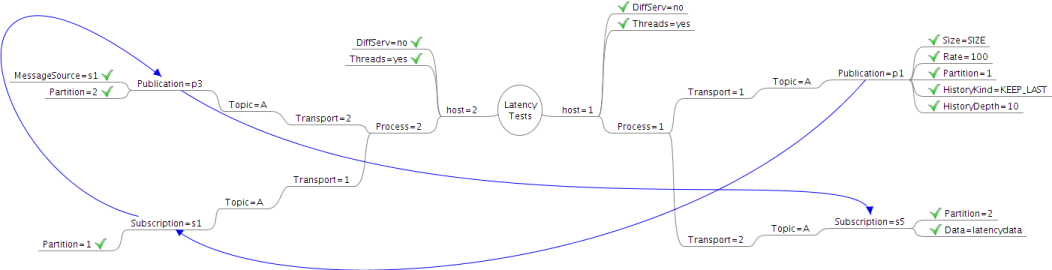
\includegraphics[width=1\textwidth]{openDDS-latency-tests}
	\caption{\label{fig:test-topology}Latency test topology
	\cite{openDDS-test-topology}}
\end{figure}

For this experiment I used one laptop HP EliteBook 2540p with the following parameters: 

\begin{itemize}
	\item CPU: Intel(R) Core(TM) i5 CPU M 540 locked at 1.2GHz frequency
	\item Memory: SAMSUNG 8GB 2x4GB PC3-10600 DDR3 1333MHZ
	\item Operating System: Fedora 27 64-bit
	\item Swappiness: 0
	\item Used compiler: gcc version 7.2.1 20170915 (Red Hat 7.2.1-2) (GCC)
	\item CMake: version 3.9.6
	\item OpenDDS version 3.12 (commit: 3057ef9dbb032bc51895f70e5c350af4b10093fa) 
	\item eProsima Fast RTPS (commit: bec4a979c088a1f978af3dfdea2a72ae2a78b52a)
\end{itemize}

The dependent variable of latency will be measured with \textit{Round-Trip time} and the divided by two. This will represent a latency of a message from a publisher to a subscriber. I will discard first 1000 time measurements and then collect next 10 000 measurements of \textit{Round-Trip time} divided by two. This process will repeat for every message size which is the first independent variable. The sizes of a message will be 16,32,64,128,256,512,1024,2048,4096,8192 and 16384 bytes. The second independent variable is transport type. I will collect data for both possible transport types which are "Reliable" and "Best effort". Both types uses datagram (UDP/IP) but "Reliable" type uses also RTPS ACKs/NACKs.

After all data is collected, I will calculate mean, max, min and standard deviation from 10 000 samples for every message size and transport type. Then I also perform T-tests that should reveal if there is any statistical difference in latency performance of those two libraries.

\section{Results}
\label{sec:results}

Present the results. A good way to organise this is via subsections
for each hypothesis you tested. Include graphs of results
(e.g.\ Figure~\ref{fig:data}), tests of significance, etc. If you have
negative results, include them. A negative results is just as
informative and useful as a positive one, sometimes more so.

Guide length: 500 words.



\section{Discussion}
\label{sec:discuss}

What do the results say? What have you learned from the
experiments? Have you identified a correlation between variables, or
causation? What are the limitations of what you've done? What further
experiments might be of benefit?

Guide length: 400 words.

\section{Conclusion}
\label{sec:conc}

What have you done and why? What have you shown through your
experiments?

Guide length: 100 words.

\bibliography{myrefs}

\end{document}
